\section{Liquid $^3$He target system} 
To gain larger luminosity, a liquid target was employed and a cryogenic target system was developed for the current experiment based on the liquid $^4$He target\cite{Sato2009233}. A schematic drawing of the liquid $^3$He cryostat is shown in Fig. \ref{lhe3:cryo} and the details can be found in Ref. \cite{Iio:2012ts}.

The experimental requirements for the target system are stable heat transport to the target cell located at the center of the cylindrical detector system and thin and low-Z materials around the target to suppress the energy loss effect. The former was achieved by an L-shape cryostat and and a siphon method with two pipes connecting between cooling part and the target cell. For the latter requirement, a target cell made by beryllium and a vacuum chamber made by carbon fiber reinforced plastic (CFRP) were employed. 


\begin{figure}[]
\begin{center}
\includegraphics[width=\columnwidth]{lhe3-cryo.eps}
\caption{ \label{lhe3:cryo}
Schematic drawing of the liquid $^3$He cryostat.
}
\end{center}
\end{figure}
\begin{figure}[]
\begin{center}
\includegraphics[width=8cm]{fig/targetcell.eps}
\caption{ \label{fig-cell}
Schematic drawing of the target cell.
}
\end{center}
\end{figure}

\subsection{Cooling mechanism} 
The major cryogenic component is divided into three sections: a $^4$He separator,  a $^4$He evaporator, and  a heat exchanger between $^3$He and $^4$He.
The target cell is connected to the bottom of the heat exchanger with two 1~m long pipes. To reduce the radiation from room temperature components, all low-temperature parts are covered with a radiation shield anchored to the liquid nitrogen tank (LN$_2$ tank). 

A cooling power is generated by an evacuation of $^4$He in the evaporator with a rotary pump. The rotary pump has a pumping speed of 120 m$^3$/h, resulting in a heat-removal capability of 2.5 W at 2 K. The cooling power was used to liquify $^3$He gas at the heat exchanger. The scarce $^3$He gas is controlled by a gas-tight handling system (leak rate less than 10$^{-10}$ Pa$\cdot$m$^3$/sec).
An effective heat transport to the 1~m apart target cell was accomplished by the application of the {\it siphon method} as described in Ref. \cite{Iio:2012ts}, which uses convection of the liquid $^3$He. The liquid $^3$He warmed by the heat load inside the target cell returns to the heat exchanger through an upper pipe while $^3$He is cooled again in the heat exchanger and fed to the target cell through the lower pipe. 

\subsection{Target cell}
Figure \ref{fig-cell} shows the target. The side wall of the target cell is made of pure beryllium (more than 99.4\% purity) of 0.3 mm thick. The caps of both ends are made by AlBeMet, which is an alloy of aluminum and beryllium.% \cite{albemet}.  
The volume of the target cell is 0.48 $\ell$ in which the volume of 269 $\ell$ gaseous $^3$He at room temperature is necessary to fill up with liquid at 1.3 K.

%\subsection{Operation and performance} 
%%operation
\if0
%%% one shot %%%
For long-term operation, it is essential to reduce the total amount of $^4$He consumed. This is because exchanging the $^4$He Dewar causes significant experimental dead time. 
To minimize the $^4$He consumption, we adopted {\it one-shot} operation. 
This operation consists of two modes:
(I) the evaporator is filled up with liquid $^4$He supplied from the separator. (II) The $^4$He supply is stopped until the evaporator becomes empty. 
The operational procedure consists of a repetition of these two methods, and 
this reduces the total liquid $^4$He consumption due to the minimization of the transfer loss to the cryostat. 
The operational performance of the target system is described in the following subsection.
%%%%%%%%%%%%%%%%%%%%%%%%%%%%%%%%%%%%%%%%%%%%%%%%%%%%%%%%%%%%%%%%%%%%%%%%%%%%%%
\fi

%\subsubsection{Vacuum chamber} 
%A vacuum chamber was specially designed to reduce multiple scattering of secondary charged particles.
%As a result of the development in KEK \cite{Sato09}, the material of the vacuum chamber was carefully selected to Carbon Fiber Reinforced Plastic (CFRP) in the region covering the acceptance of the CDS. 
%The detail of the specification of adopted CFRP is found in Ref. \cite{Iio12}.
%Total thickness of the CFRP in the E15 setup is 1 mm with the diameter of 150 mm and the length of 523 mm. 
% An aluminum beam window with the thickness of 0.6 mm is glued to the CFRP with STYCAST 1266.
%A safety factor of this vacuum chamber is estimated to be 3.8 against the external pressure of 1 atm. 

\subsection{Operation and performance\label{sec-target}} 
After a pre-cooling of the cryogenic system to the liquid nitrogen temperature, it took about 6 hours to liquify the $^3$He gas in the heat exchanger and achieve thermal equilibrium at around 1.4 K.  

Figure \ref{fig-lheope}(left) shows the stability of the temperature at the target cell during the experiment. The spike-like temperature rises are the periods when we refilled the liquid $^4$He to the evaporator.  We need to refill the $^4$He once per about 24 hours and it takes about 1 hour including a recovery time to thermal equilibrium. Liquid $^4$He at 4.2 K is transported to the evaporator through the separator, which is closed off during the normal operation. 
In the data taking period, the temperature was in the range between 1.37 and 1.44 K, which corresponds to the density fluctuation of $\sim$ 0.2\% as the density equation of $^3$He is shown in Fig. \ref{fig-lheope}(right)\cite{Huang:2005ge}. Since the equilibrium temperature of $\sim$1.4 K was $\sim$ 0.1 K higher than that of the test operation in Ref. \cite{Iio:2012ts}, the difference was also taken into account for the uncertainty of the density. Then, the liquid $^3$He density in the experimental period was evaluated to be is 0.0810$\pm$0.0002~g/cm$^3$, corresponding to a thickness of 1.11~g/cm$^2$ for 138 mm length along the beam direction.
The temperature differences between the evaporator, the heat exchanger, and the target cell were less than 0.01 K. This means that the heat transfer by the {\it siphon method} was working well. From the reduction rate of the liquid $^4$He in the evaporator, the heat load of the low-temperature region was estimated to be 0.21 W. The operational results of the cryostat are tabulated in Table \ref{operation}.

\begin{table}[] 
\begin{center}
\caption{\label{operation}Operational results of the liquid $^3$He target system.}
\begin{tabular}{lrc}\hline\hline
Vacuum level                      & [mbar]                 &$ < 10^{-6}$ \\ 
Leak rate of the $^3$He system    & [Pa$\cdot$m$^3$/sec] &$< 10^{-10}$ \\ 
Temperature in the target cell    &[K]       & 1.4        \\
Vapor pressure in the target            &[mbar]    & 33         \\
Heat load to low-temperature part   &[W]       & 0.21       \\ 
Liquid $^4$He consumption          &($\ell$/day)      & 50         \\ 
Liquid N$_2$ consumption          &($\ell$/day)      & 50         \\ 
 \hline \hline  
\end{tabular}
\end{center}
\end{table}

\begin{figure}[]
\begin{center}
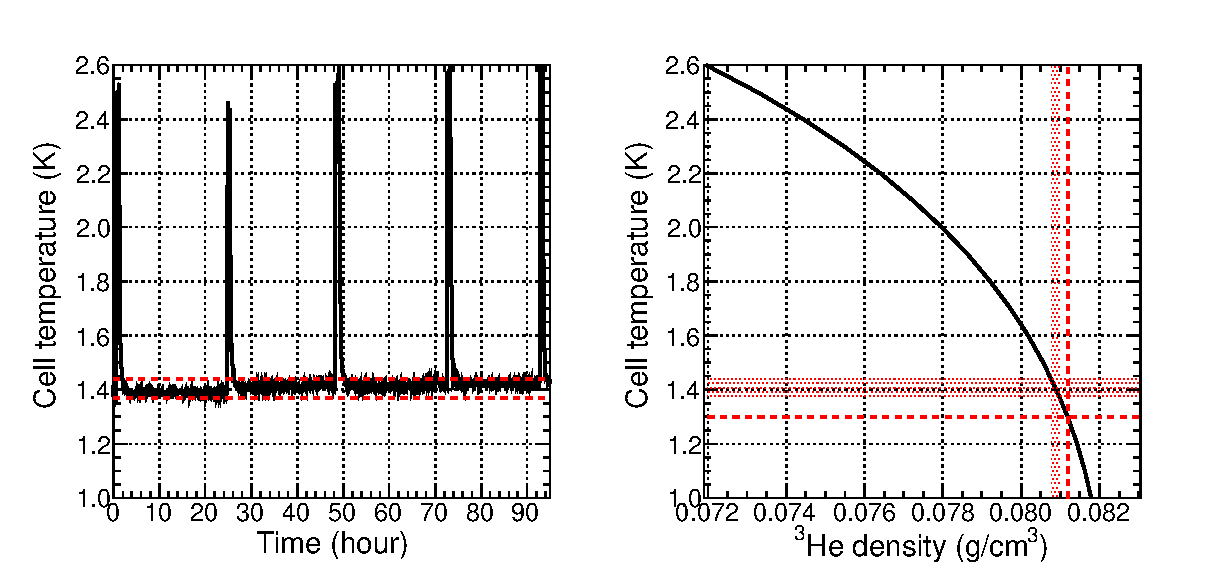
\includegraphics[width=\columnwidth]{fig/target-temp.eps}
\caption[Stability of the target temperature and its effect to the target density.]{ \label{fig-lheope}
(left) Stability of the temperature at the target cell during the experiment. (right) Density equation of $^3$He\cite{Huang:2005ge}. The hatched regions represent the uncertainty caused by the temperature measurement. The dotted line represents the result in Ref. \cite{Iio:2012ts}.
}
\end{center}
\end{figure}

%%%  References
% M. Iio et al., submitted to Nucl. Instr. and Meth. A
% M. Sato et al., Nucl. Instr. and Meth. A 606 (2009) 233 
